% !TEX root = ../ausarbeitung.tex

\chapter{Evaluation}

Die Applikation wurde mit dem Hauptziel entwickelt, eine Nutzeroberfläche zu bieten, mit der sowohl Personen, die in der LRS Therapie arbeiten (wie LerntherapeutInnen oder Lehrkräfte) als auch Nicht-ExpertenInnen (z.B. die Eltern betroffener Kinder) intuitiv und effizient benötigtes Arbeitsmaterial erstellen können. Außerdem wurde untersucht wie eine Datenbank für Betonungsmuster in Wörtern erstellt und benutzerfreundlich erweitert werden kann.

Die Evaluation untersucht daher folgende Punkte:
\begin{itemize}
	\item Erstellung von Arbeitsmaterial aus einem Fließtext
	\item Intuitivität und Einfachheit der Bedienung
	\item Effizienz des Prozesses der Erstellung von Arbeitsmaterial
	\item Nutzerfreundliche Erweiterung der Wortdatenbank
\end{itemize}

Zunächst wird durch Beispiele eines annotieren Textes mit verschiedenen Einstellungen demonstriert, welche vielseitigen Möglichkeiten die Textannotation für das Erstellen von Arbeitsmaterial bietet. Für die Untersuchung von Intuitivität, Einfachheit und Effizienz bei der Bedienung der Applikation wurde ein Nutzertest durchgeführt. Dieser fand als Interview statt um qualitative Daten durch Nutzerbefragung zu erheben. Außerdem wurden quantitative Daten durch das Ausfüllen von Ankreuzfragen während des Interview erhoben.

\section{Ergebnisse der Textannotation}
\label{sec:annotation-results}

Um zu zeigen, dass die Applikation das Ziel des automatischen Erstellens von Arbeitsmaterial erfüllt, werden im Folgenden verschiedene Texte präsentiert, die mit Hilfe des Web Interfaces erstellt wurden. Die Ergebnisse zeigen, dass das Programm dieses Ziel nicht nur erfüllt, sondern im Vergleich zu herkömmlichen Methoden auch noch einen hohen Grad an Flexibilität bietet. Die Einstellungen und damit das Erscheinungsbild des resultierenden Textes können von der Nutzerin oder dem Nutzer frei an die Bedürfnisse des jeweiligen Falls angepasst werden.

Im Folgenden wurde der Beispieltext \textit{Aschenputtel} (s. Abschnitt \ref{sec:anhang-test} im Anhang) mit der Web Applikation analysiert, sodass Silbentrennung und Betonung farblich markiert dargestellt wurden. Die in den Beispielen verwendeten Texten wurden mit der Druckfunktion der Textvorschau als PDF Dateien exportiert. Jedes Bild entspricht einer DIN A4 Seite.

\subsubsection{Beispiel 1: Hervorhebung der Silben mit zwei alterierenden Farben}

Im ersten Beispiel wird die Schriftfarbe für das Hervorheben der Silben genutzt. Die betonte Silbe wird immer rot dargestellt, in Wörtern mit vielen Silben werden diese dann alterierend rot und blau hervorgehoben. Die Schriftgröße wurde auf \textit{22} gesetzt, der Wortabstand auf den Wert \textit{0.4}. Zusätzlich sorgt die Einstellung des Zeilenabstands mit dem Wert \textit{1.5} für bessere Lesbarkeit.

\begin{figure}[h!]
	\centering
	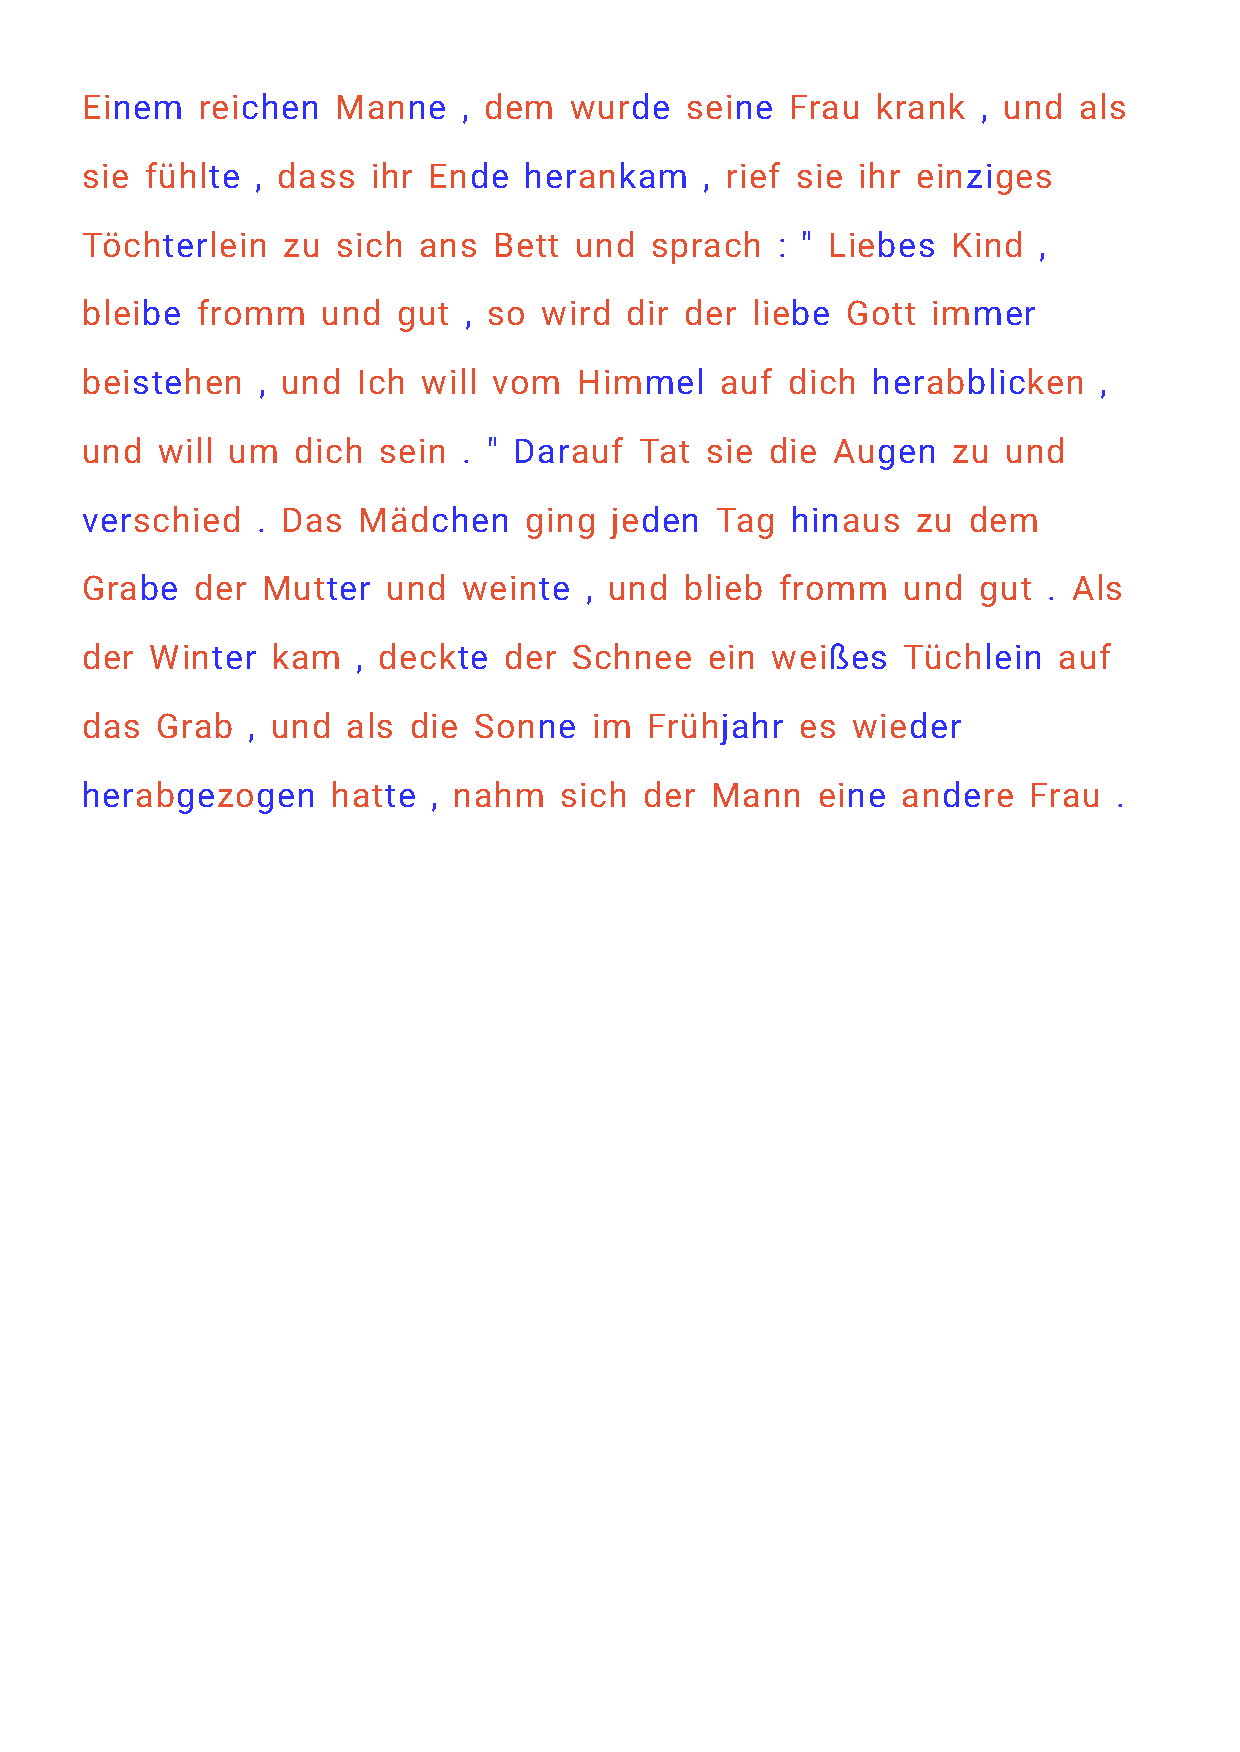
\includegraphics[width=.7\linewidth, frame]{figures/evaluation/annotation1}
	\caption{Hervorhebung der Silben mit zwei alterierenden Farben}
	\label{fig:evaluation-ex1}
\end{figure}
\newpage

\subsubsection{Beispiel 2: Worthintergrund und Silbenabstand}

In diesem Beispiel sorgt die Worthintergrundfarbe für eine bessere Wahrnehmung des Wortes als Einheit. Dadurch kann auch ein Silbenabstand (hier \textit{0.1}) eingestellt werden ohne dass die Gefahr besteht, dass dadurch nicht mehr klar ist, welche Silben zusammen gehören. Wegen dem Worthintergrund nehmen die Wörter mehr Platz in der Zeile ein, daher wurde auch der Zeilenabstand auf \textit{2.2} erhöht. Zudem wurde hier ein Zeichenabstand von \textit{2} (statt \textit{1} in Beispiel 1) gewählt.

\begin{figure}[h!]
	\centering
	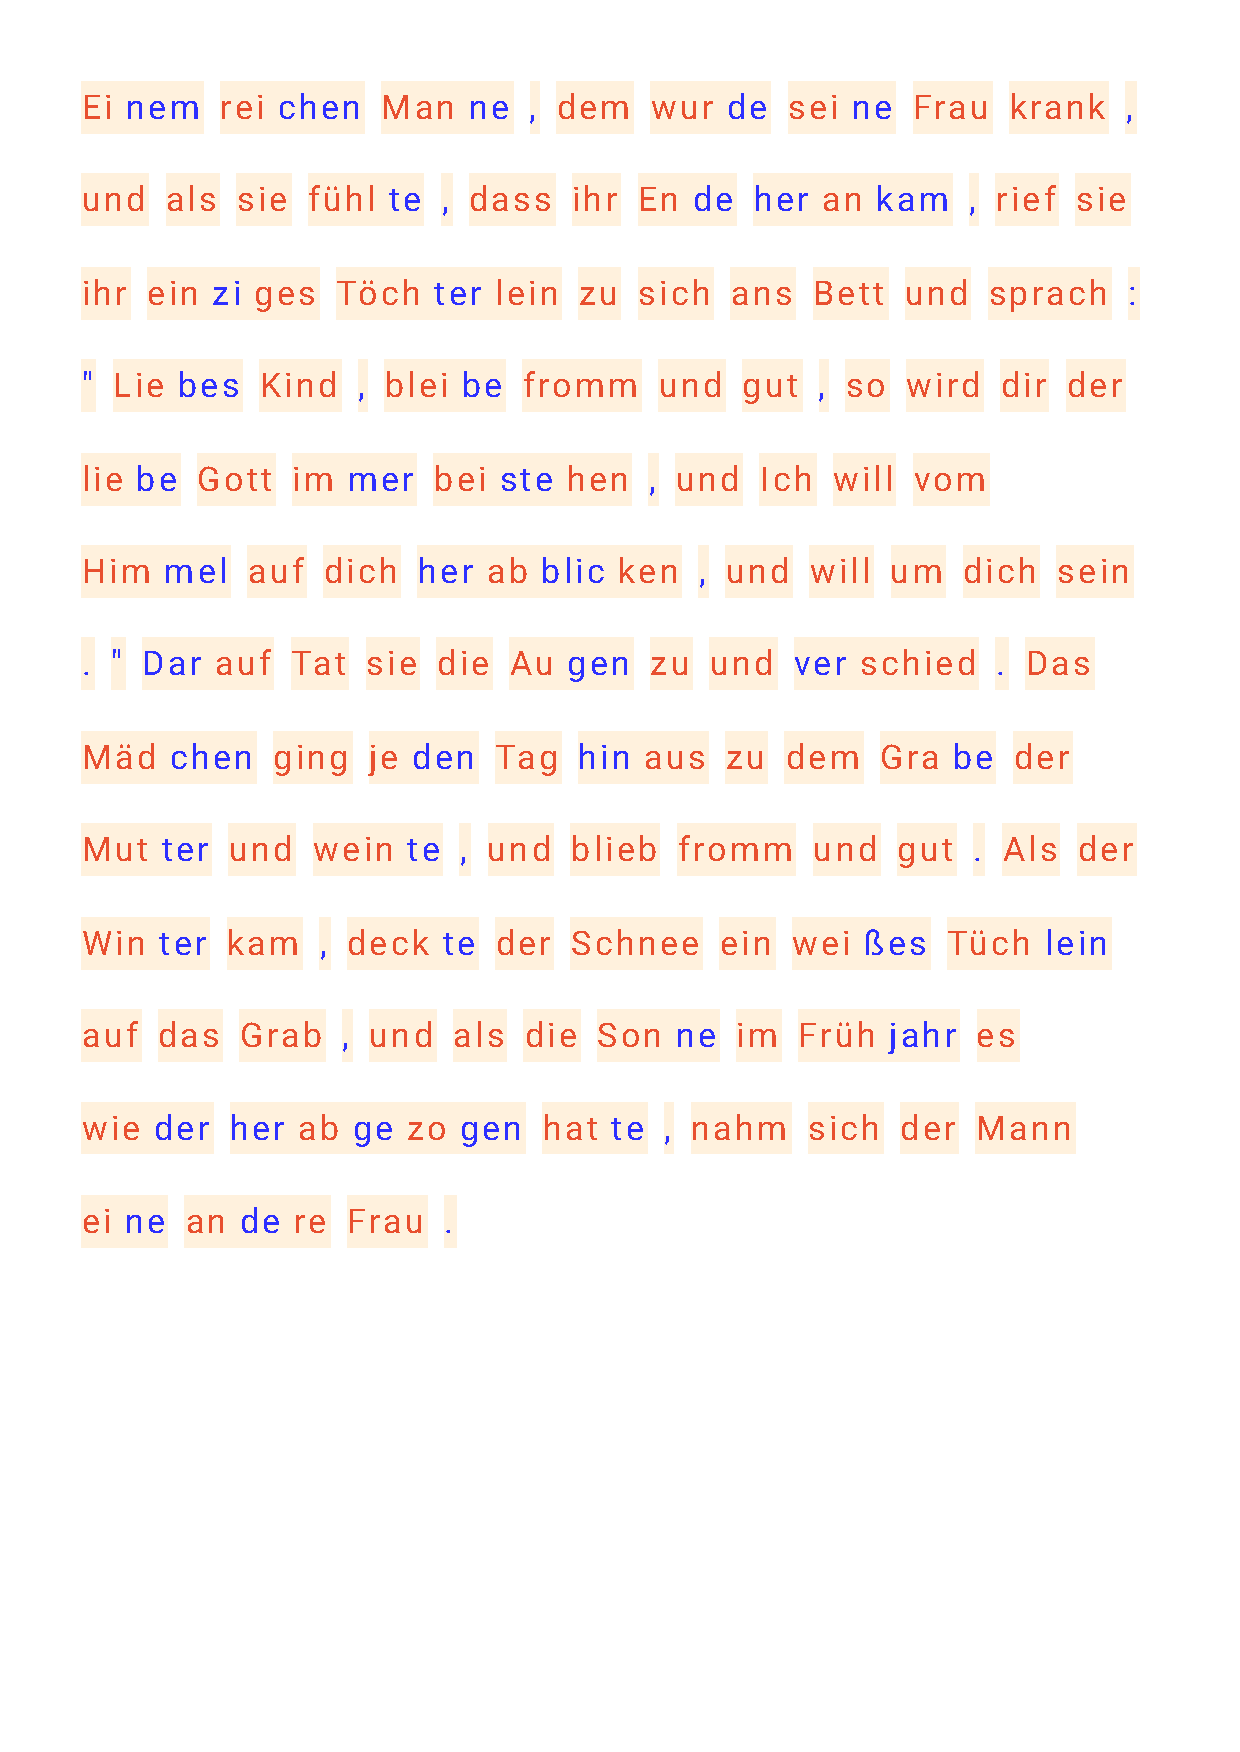
\includegraphics[width=.7\linewidth, frame]{figures/evaluation/annotation2}
	\caption{Worthintergrund und Silbenabstand}
	\label{fig:evaluation-ex2}
\end{figure}
\newpage

\subsubsection{Beispiel 3:  Silbentrennzeichen und verschiedene Silbenfarben}

In Beispiel 3 wurde wieder auf die Worthintergrundfarbe verzichtet. Das Trennzeichen \qq{=} soll hier das Silbentrennen erleichtern, sowie zusammenhängende Silben zu einem Wort gruppieren. Der Zeichenabstand beträgt wieder \textit{1}, der Silbenabstand \textit{0}, da das Gleichheitszeichen hier als Silbentrenner dient. Zusätzlich wurde eine weitere Farbe für alterierende Silben gewählt. Hier wird nur noch die betonte Silbe rot dargestellt, danach alterieren die Silben bei langen Wörtern in den Farben blau und lila.

\begin{figure}[h!]
	\centering
	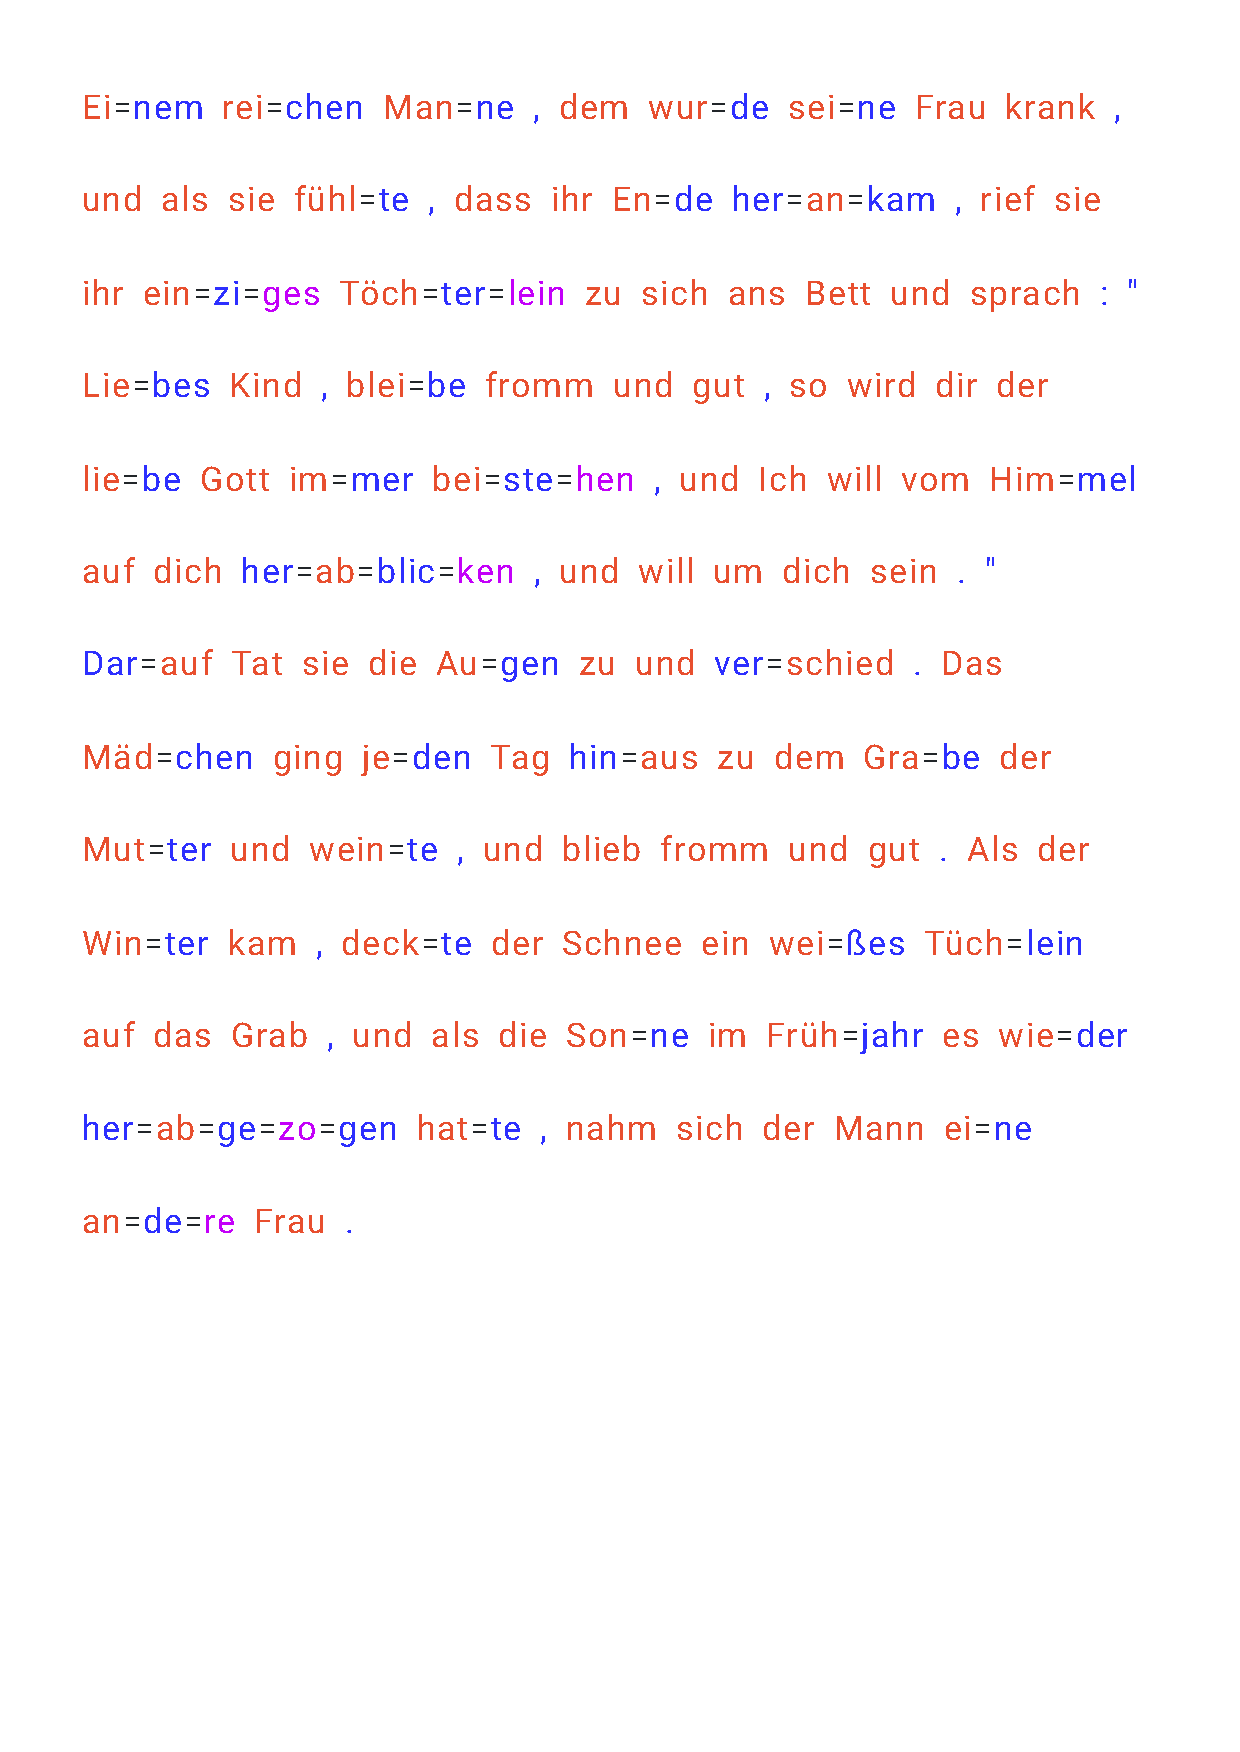
\includegraphics[width=.7\linewidth, frame]{figures/evaluation/annotation3}
	\caption{Silbentrennzeichen und verschiedene Silbenfarben}
	\label{fig:evaluation-ex3}
\end{figure}
\newpage

\subsubsection{Beispiel 4: Hervorhebung des Silbenhintergrunds}

In diesem Beispiel wird ein anderer Ansatz der farblichen Hervorhebung gewählt. Die eingestellten Farben bestimmen hier den Hintergrund der Silben und nicht die Schriftfarbe (diese ist immer Schwarz). Das Beispiel hebt vor Allem die betonte Silbe hervor, die grün dargestellt werden. Unbetonte Silben bekommen alterierend zwei verschiedene Grautöne als Hintergrund. Der Silbenabstand ist hier wieder \textit{0}, somit wird die Einheit des Wortes deutlich erkennbar.

\begin{figure}[h!]
	\centering
	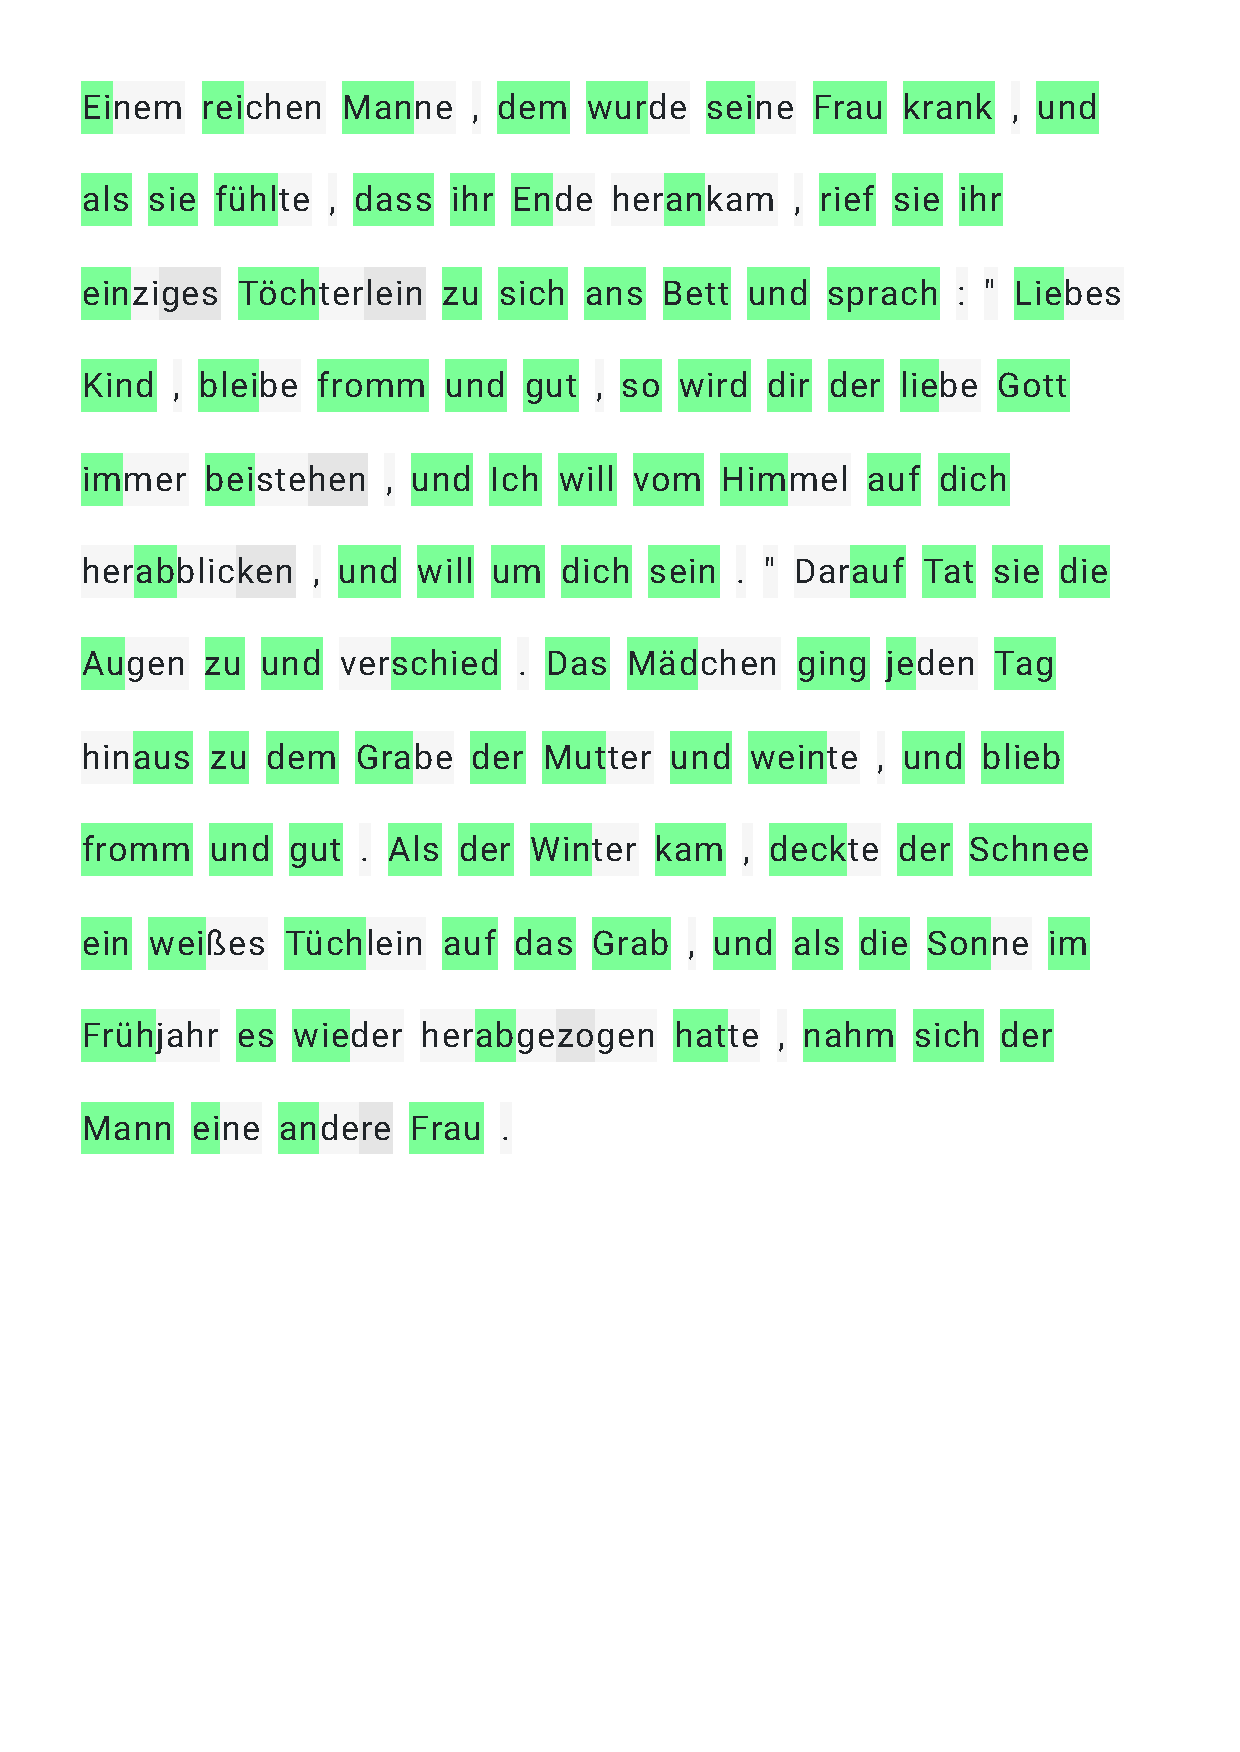
\includegraphics[width=.7\linewidth, frame]{figures/evaluation/annotation4}
	\caption{Hervorhebung des Silbenhintergrunds}
	\label{fig:evaluation-ex4}
\end{figure}
\newpage

\subsubsection{Beispiel 5: Manuelles Deaktivieren der Hervorhebung in kurzen Wörtern}

In Beispiel 5 wird der Sprachrhythmus mit Wortbetonungen noch deutlicher hervorgehoben. Die betonte Silbe wird zusätzlich zur grünen Farbe auch fett dargestellt. Außerdem wurde die Betonung in manchen Wörtern deaktiviert, so werden im ganzen Text beispielsweise Artikel, Präpositionen oder manche einsilbigen Wörter nicht betont markiert. Dieser Text soll damit einen Fokus auf den Sprachrhythmus innerhalb ganzer Sätze legen.

\begin{figure}[h!]
	\centering
	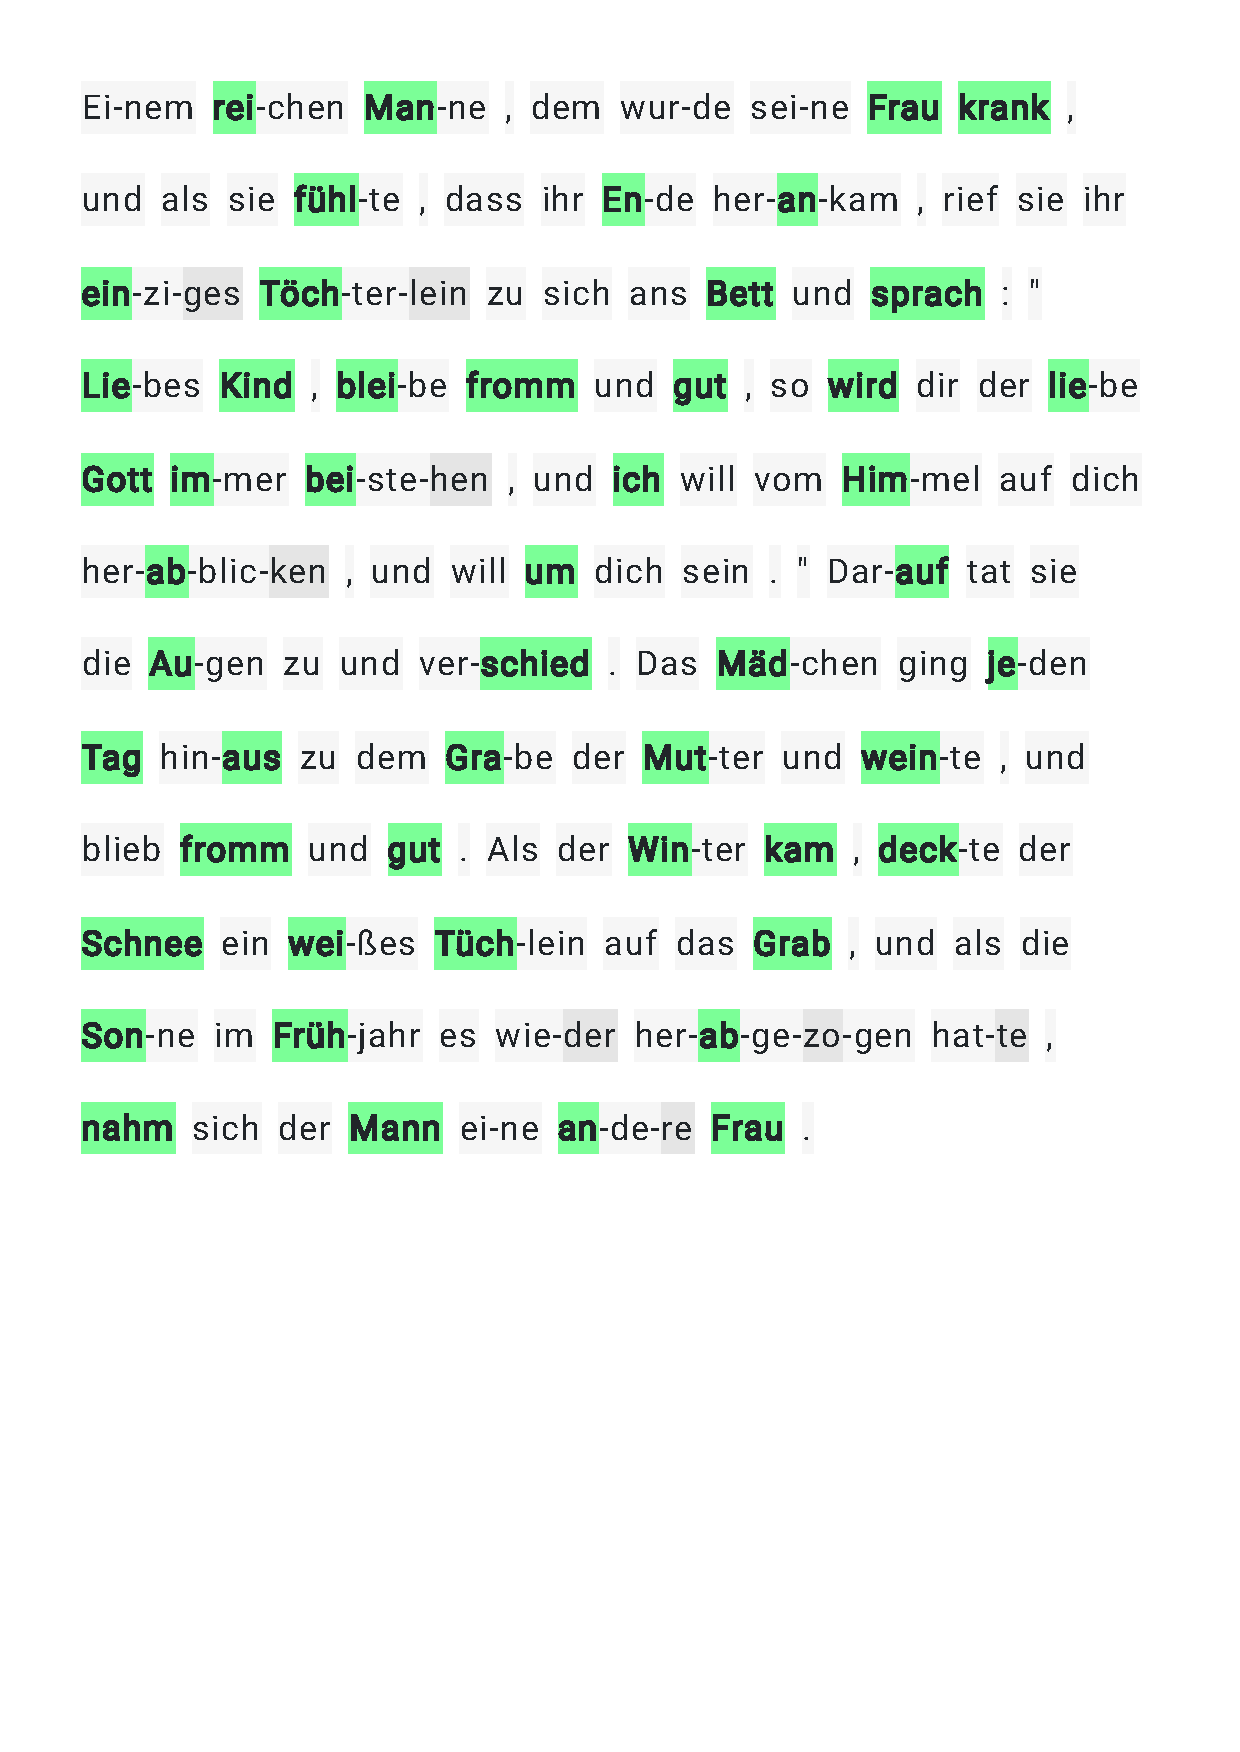
\includegraphics[width=.7\linewidth, frame]{figures/evaluation/annotation5}
	\caption{Manuelles Deaktivieren der Hervorhebung in kurzen Wörtern}
	\label{fig:evaluation-ex5}
\end{figure}
\newpage

\section{Nutzertest}
\label{sec:usertest}

Während die Beispiele im vorherigen Abschnitt verdeutlichen, dass die entwickelte Applikation generell dazu in der Lage ist Texte anforderungsgemäß zu annotieren, sollte der Nutzertest zeigen, ob die Applikation von der Zielgruppe (LerntherapeutInnen, Lehrkräfte und Eltern betroffener Kinder) problemlos bedient werden kann. Intuitivität und Zeiteffizienz sollten dabei vor Allem berücksichtigt werden, da Software, die diese Kriterien schlecht erfüllt, ungern oder im schlechtesten Fall überhaupt nicht benutzt wird.\\
Vor dem eigentlichen Nutzertest wurde zunächst ein Pilottest durchgeführt. Dieser half dabei, Mängel im Design des Tests an sich aufzudecken und Fehler in der Webapplikation zu finden, welche keinen direkten Einfluss auf die Usability hatten und die noch vor dem Nutzertest behoben werden konnten.

\subsection{Vorbereitung und Durchführung}

Der Nutzertest beinhaltete neben den statistischen Daten zu Alter und Beruf bzw. Studiengang fünf Szenarien, die die NutzerInnen bearbeiten sollten. Um detaillierte Informationen zur Vorgehensweise der ProbandInnen zu erhalten, wurde im Interview mit der \textit{Thinking Aloud} Methode gearbeitet, d.h. die Testperson wurde aufgefordert bei jeder Aktion, die sie durchführt, möglichst genau zu beschreiben was sie damit bezweckt und warum sie es tut\cite{Nielsen1993}. In der schriftlichen Testbeschreibung wurden die NutzerInnen daher informiert, alle Arbeitsschritte der Szenarien laut vorzulesen und Kommentare und Kritik jederzeit zu äußern. Außerdem wurde in jedem Text explizit mündlich darauf hingewiesen, alle Handlungen möglichst genau zu beschreiben. In der Testbeschreibung wurde auch verdeutlicht, dass es sich um ein Test des Softwaresystems handelt und nicht der Nutzerin oder des Nutzers.

Um möglichst konsistente Testbedingungen zu schaffen, wurde bei allen ProbandInnen mit einer aktuellen Version von Google Chrome gearbeitet. Es wurde zudem sichergestellt, dass den Testpersonen ein möglichst gewohntes Umfeld geboten wird. Im besten Fall benutzten die NutzerInnen ihre eigenen Computer. Falls dies nicht möglich war, wurde vorher überprüft ob beim Testgerät alles genauso wie gewohnt bedient werden konnte, d.h. Einstellungen für Peripherie wie Maus, Tastatur oder Touchpad wurden vorher, der Nutzerin oder dem Nutzer entsprechend angepasst.

Nach jedem der fünf Szenarien wurde von den ProbandInnen ein \textit{After Scenario Questionnaire}\cite{Lewis1995}. Es beinhaltete die folgenden drei Fragen:
\begin{itemize}
	\item \textbf{Intuitivität}: \qq{Die Aufgabe konnte ich intuitiv und problemlos erledigen.}
	\item \textbf{Zeitaufwand}: \qq{Ich halte die Zeit, die ich gebraucht habe um die Aufgabe zu erledigen, für angemessen.}
	\item \textbf{Dokumentation}: \qq{Ich bin mit den Informationen, die ich während der Bearbeitung in der App erhalten habe (Beschreibungen, Rückmeldungen) zufrieden.}
\end{itemize}

Zustimmung oder Ablehnung konnte für jede Aussage in den fünf Optionen \textit{trifft zu}, \textit{trifft eher zu}, \textit{weder noch}, \textit{trifft eher nicht zu} oder \textit{trifft nicht zu} ausgedrückt werden.

Die Software wurde insgesamt 7 ProbandInnen getestet, wobei bei der Auswahl darauf geachtet wurde, dass die  Applikation den Testpersonen unbekannt war (sie also die Applikation nicht vorher schon bedient hatten). Die Befragten wurden in zwei Gruppen eingeteilt, zum Einen die Expertengruppe, bestehend aus Lerntherapeutinnen, und zum Anderen die Laien, die exemplarisch für Menschen (z.B. Elternteile) aus dem Umfeld der Betroffenen stehen. Durch die Befragung von Experten wurde eine besonders kritische, realistische und fachbezogene Einschätzung der Software erhofft. Es wurden 3 Expertinnen und 4 Laien befragt. Das Alter der ProbandInnen lag zwischen 22 und 51 Jahren (Durchschnitt 34 Jahre). 5 Versuchspersonen waren Frauen, 2 waren Männer.\\

\subsection{Ergebnisse}

Im Folgenden werden die einzelnen Szenarien beschrieben und deren Ergebnisse dargestellt. Von den ProbandInnen erkannte und während des Szenarios geäußerte Schwierigkeiten und Probleme werden hier jeweils kurz zusammengefasst und im Anhang (Abschnitt \ref{sec:anhang-test}) tabellarisch, zusammen mit eventuellen Vorschlägen zu deren Behebung im Anhang aufgelistet.

\subsubsection{Szenario 1: Nutzerkonto}

Zuerst sollte die Testperson ein Nutzerkonto mit Mailadresse und Passwort erstellen (hier wurde, damit die Testperson kein sicherheitskritisches Passwort verwendet und sich das Passwort während des Tests merken kann \qq{12345678} vorgegeben). Anschließend loggte sie sich ein und wieder aus.

\begin{figure}[h!]
	\centering
	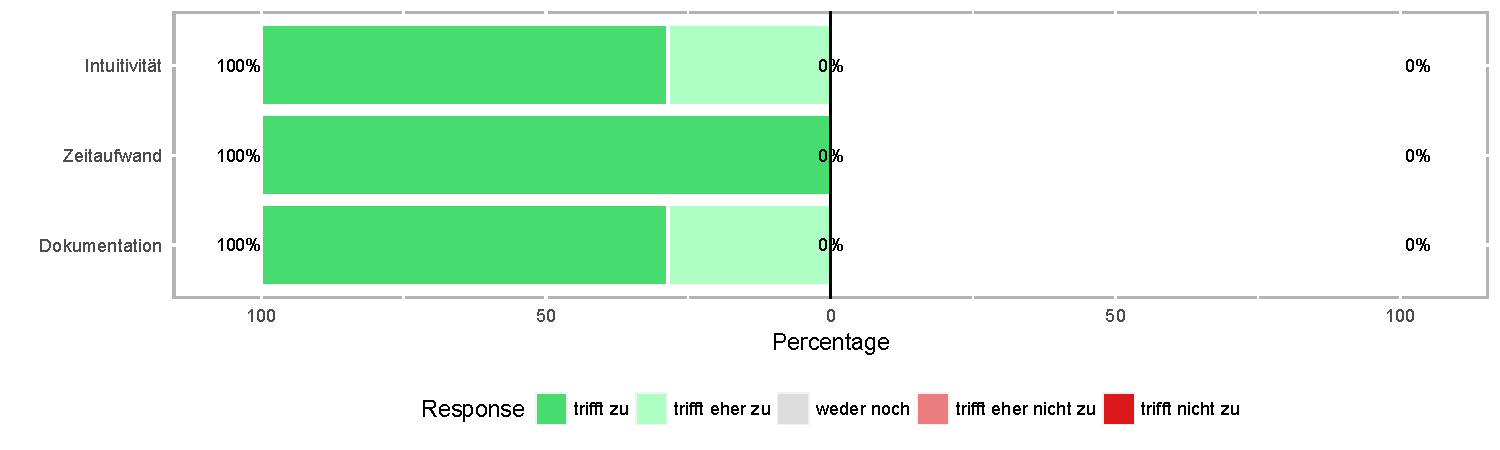
\includegraphics[width=.8\linewidth]{figures/evaluation/scenario1}
	\caption{Quantitative Ergebnisse von Szenario 1 (Nutzerkonto)}
	\label{fig:evaluation-sc1}
\end{figure}

Die Testpersonen konnten die Aufgabe meist problemlos lösen. Mehrmals wurde vor dem Erstellen des neuen Kontos erst Mailadresse und Passwort in das Login Fenster eingetragen, was zu einer Fehlermeldung führte (da das Konto noch nicht existierte). Die Testpersonen kamen aber in jedem Fall selbst darauf, dass man dem Link \textit{Neues Konto erstellen} folgen musste. Hier könnte die Unterscheidung zwischen Login und Konto erstellen noch deutlicher gemacht werden, bzw. könnte der Link zum Konto erstellen besser sichtbar platziert werden (s. Tabelle \ref{table:szenario1} im Anhang).

\subsubsection{Szenario 2: Textanalyse}

Als nächstes loggte sich die Testperson wieder ein und sollte einen gegebenen Text in das Textfeld der Textanalyse kopieren und diesen dann analysieren lassen. Alle unbekannten Wörter (in der Anwendung rot hinterlegt) sollten anschließend manuell geklärt werden. Die NutzerInnen klickten so lange durch das User Interface der manuellen Analyse, bis alle Wörter annotiert waren. Als Letztes sollte mit den Einstellungen der Annotation experimentiert werden, bis eine Einstellung gefunden wurde, welche die Testperson ansprach. Hier wurde noch mündlich hinzugefügt, dass um sich damit vertraut zu machen, alle Einstellungen einmal ausprobieren werden sollten.

\begin{figure}[h!]
	\centering
	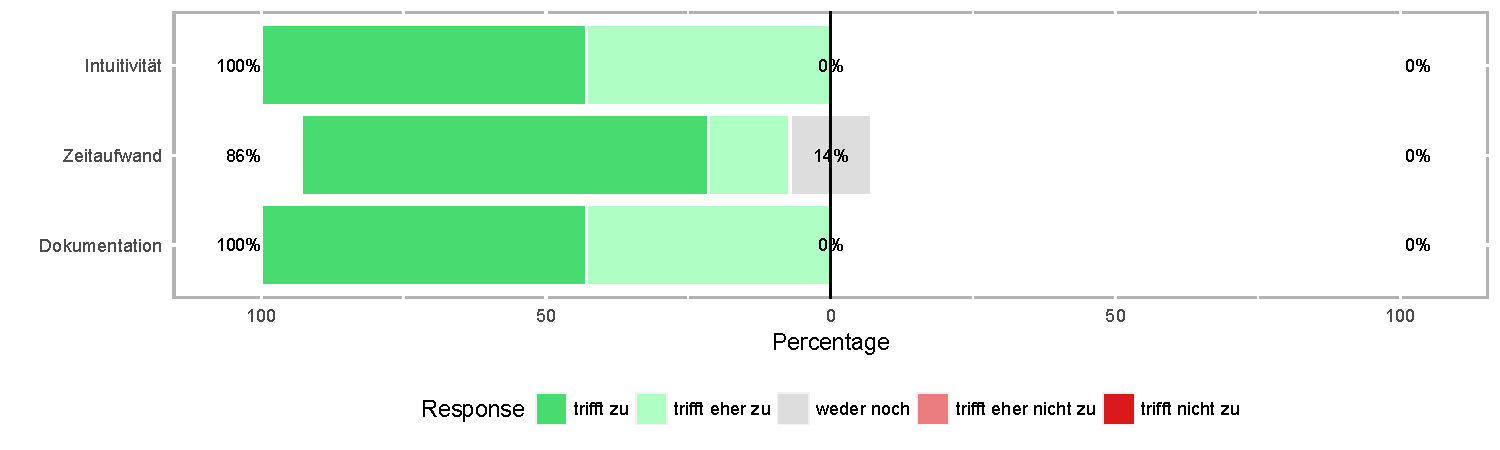
\includegraphics[width=.8\linewidth]{figures/evaluation/scenario2}
	\caption{Quantitative Ergebnisse von Szenario 2 (Textanalyse)}
	\label{fig:evaluation-sc2}
\end{figure}

Auch hier konnten alle Testpersonen die Aufgabe bewältigen. Es wurde teilweise das Layout bemängelt. Es war umständlich, Einstellungen zu verändern, wenn man dafür weit runter scrollen musste und so den Vorschautext nicht mehr im Blick hatte. Hier wurde eine kompaktere Darstellung der Einstellungen gewünscht. Es wurde außerdem vorgeschlagen, die Farbauswahl zu vereinfachen, sodass dafür nicht jedes mal ein extra Fenster aufgeht (s. Tabelle \ref{table:szenario2} im Anhang).

\subsubsection{Szenario 3: Annotationsvorlagen}

Im dritten Szenario wurden der Testperson zweimal die erste Zeile des Textes, jeweils mit verschieden Einstellungen annotiert, vorgegeben. Sie sollte nun nacheinander versuchen, die Annotation so einzustellen, dass es etwa so wie im gegebenen Ausschnitt aussah. Zudem sollten diese Einstellungen als Vorlagen mit den Namen \qq{Vorlage 1} und \qq{Vorlage 2} gespeichert werden. Zum Schluss wechselte die Nutzerin oder der Nutzer zwischen Vorlage 1 und Vorlage 2 hin und her.

\begin{figure}[h!]
	\centering
	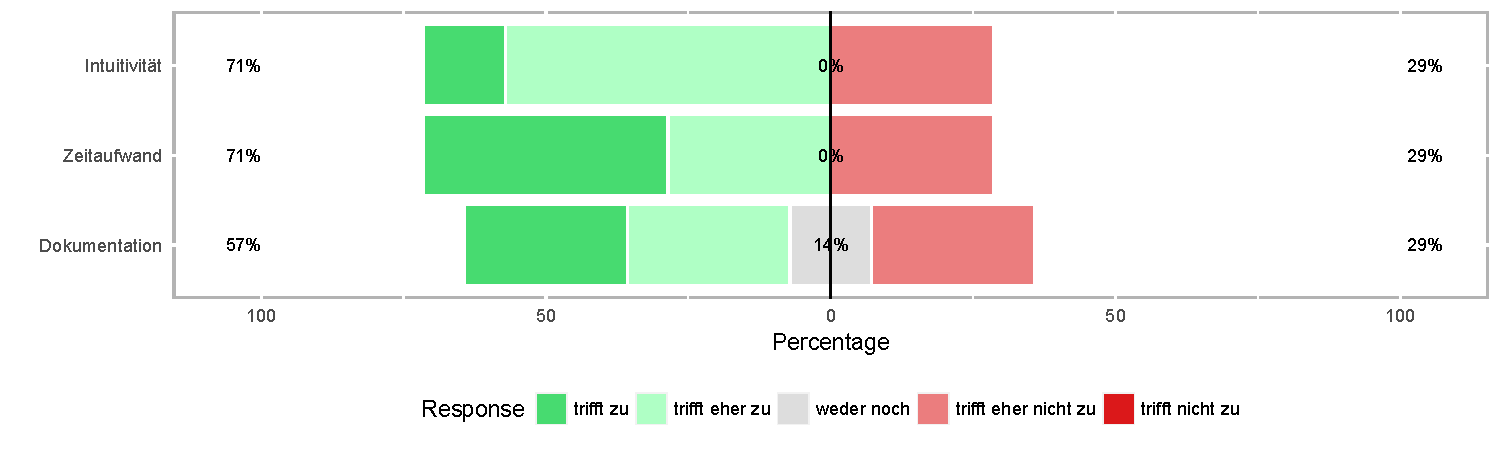
\includegraphics[width=.8\linewidth]{figures/evaluation/scenario3}
	\caption{Quantitative Ergebnisse von Szenario 3 (Annotationsvorlagen)}
	\label{fig:evaluation-sc3}
\end{figure}

Das Speichern und Wechseln der Vorlagen bereitete den Testpersonen hier großteils keine Probleme. Fast alle NutzerInnen konnten allerdings den Text für Vorlage 2 (farbiger Hintergrund mit schwarzer Schrift) nicht ohne Hilfe entsprechend anpassen. Hier war nicht klar, was die Option \textit{Silbe betonen} bedeutete und wurde oft mit der \textit{Wort Hintergrundfarbe} verwechselt. Erst durch längeres Ausprobieren oder Hilfestellungen konnten die Testpersonen die Aufgabe lösen. Hier sollte zum Einen der Aufbau und die Beschreibung der Elemente der Einstellungen überarbeitet werden, zum Anderen legen die Probleme bei den Einstellungen nahe, eine kurze Einführung (evtl. in Form einer Kurzdokumentation oder Online-Hilfe in der Applikation) bereitzustellen (s. Tabelle \ref{table:szenario3} im Anhang).

\subsubsection{Szenario 4: Texte wiederverwenden}

Hier sollte die Testperson den aktuellen Text mit Titel in ihrem Nutzerkonto speichern. Anschließen wurde auf die Nutzerkonto Seite gewechselt und der gespeicherte Text neu analysiert.

\begin{figure}[h!]
	\centering
	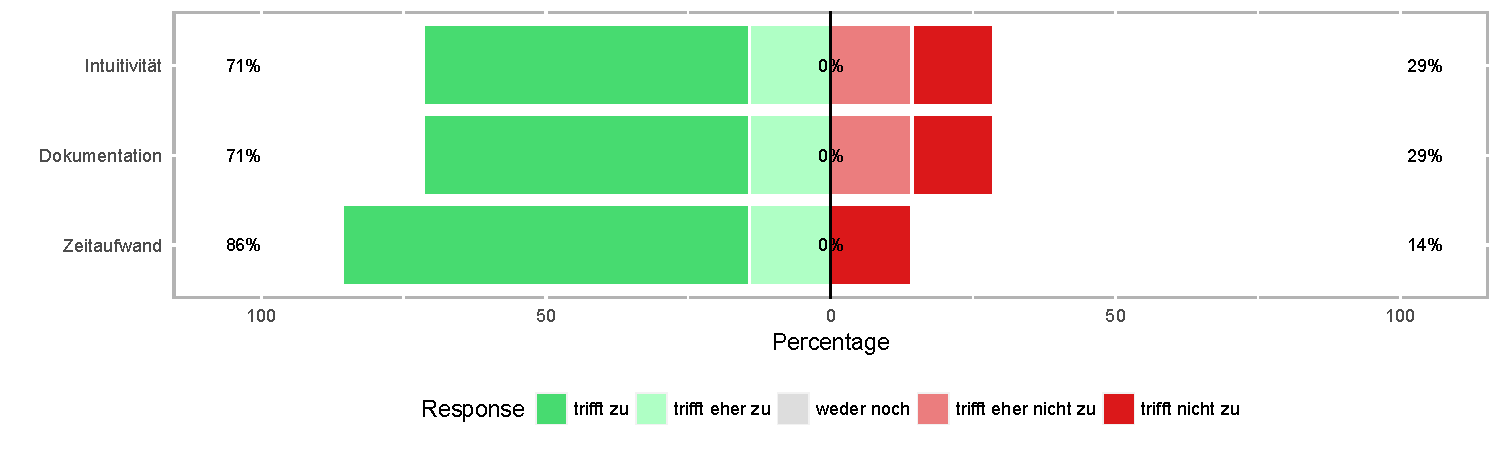
\includegraphics[width=.8\linewidth]{figures/evaluation/scenario4}
	\caption{Quantitative Ergebnisse von Szenario 4 (Texte wiederverwenden)}
	\label{fig:evaluation-sc4}
\end{figure}

Die meisten Testpersonen konnten diese Aufgabestellung problemlos lösen. Zwei Probandinnen konnten die Aufgabe allerdings nicht ohne Hilfestellung bewältigen, da die Nutzerseite nicht gefunden wurde. Hier war nicht klar, dass der Link rechts oben in der Navigation zur Nutzerkonto Seite führt und dort Nutzertexte gespeichert sind. Die Navigation könnte hier noch deutlicher und übersichtlicher gestaltet werden (s. Tabelle \ref{table:szenario4} im Anhang).

\subsubsection{Szenario 5: Wort Verifizierung}

Im letzten Szenario wechselte die Nutzerin oder der Nutzer auf die Verifizierungsseite. Hier sollten vier Einträge anderer NutzerInnen bestätigt oder verbessert werden.

\begin{figure}[h!]
	\centering
	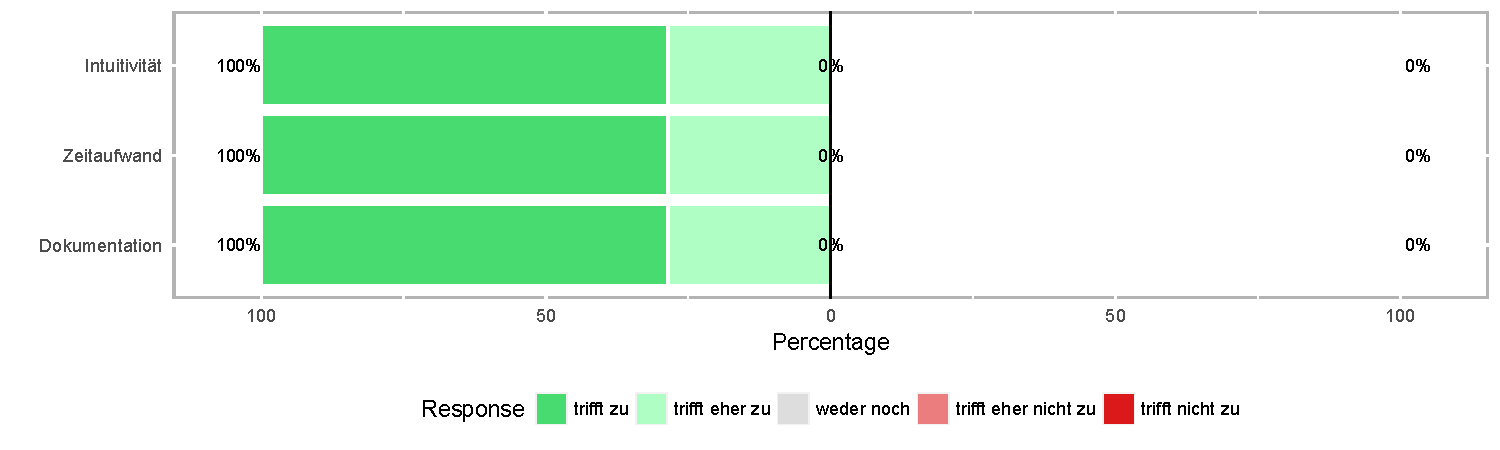
\includegraphics[width=.8\linewidth]{figures/evaluation/scenario5}
	\caption{Quantitative Ergebnisse von Szenario 5 (Wort Verifizierung)}
	\label{fig:evaluation-sc5}
\end{figure}

Bei der Durchführung der Verifizierung gab es keine größeren Probleme. In einigen Vorschlägen bemerkten die Testpersonen, dass der Prozess zum Beispiel verbessert werden könnten, indem mehrere Wörter auf einmal in einer Liste \qq{abgehakt} werden könnten oder für Änderungen bei der Segmentierung die Texteingabe für die Silbentrennung vereinfacht werden könnte (s. Tabelle \ref{table:szenario5} im Anhang).

\subsubsection{Allgemeine Anmerkungen}

Zum Schluss des Nutzertest wurden die ProbandInnen zu allgemeinen Äußerungen von Kritik und Vorschlägen zur Applikation als Ganzes aufgefordert. Wichtige Ideen und Kommentare sind im Folgenden festgehalten:

\begin{itemize}
	\item Alte, nicht mehr aktuelle Fehlermeldungen verschwinden oft nicht (oder nur, wenn man sie selbst schließt). Diese sollten sich beim Ausführen neuer Interaktionen automatisch schließen.
	\item Die \textit{Home} Seite sollte die Beschreibungen besser gruppieren (z.B. nebeneinander mit Bildern) und die Breite besser ausnutzen.
	\item Die türkise Farbe für die Umrandung der Kästen wirkte unpassend. Diese könnte in die blaue Farbe der Links geändert werden.
	\item Es wurde eine Option gewünscht, bei der die Wortbetonung in der Annotation vollständig ausgeschaltet wird und stattdessen ein einfaches, abwechselndes Einfärben der Silben (über Wortgrenzen hinaus) ermöglicht wird.
	\item Beim Navi-Link zum Nutzerkonto (Mailadresse rechts oben) könnte ein Bücherregal Symbol verdeutlichen, dass dort Nutzertexte zur Wiederverwendung gespeichert werden.
\end{itemize}

\newpage
\section{Diskussion}

In der Evaluation wurde geprüft inwiefern die Ergebnisse der mit der Applikation erstellten Texten mit den gesetzten wissenschaftlichen Zielen übereinstimmten und wie Nutzerinnen und Nutzer die Bedienbarkeit der Applikation einschätzten. Ziel der Entwicklung war es eine Applikation zu schaffen, mit der Übungstexte für die LRS Therapie einfach erstellt werden können.\\
Zum Einen zeigen die erstellten Beispieltexte (s. Abschnitt \ref{sec:annotation-results}), dass solche Texte mit der Applikation erstellt und exportiert werden können. Im Vergleich zu bereits existierenden Lösungen (s. Abschnitt \ref{sec:lrs-digital}) bietet die entwickelte Webanwendung mehr Einstellungsmöglichkeiten und ist somit flexibler in der Gestaltung der Textannotation. Neben dieser Erkenntnis sollte der Nutzertest zeigen, dass die Texte einfach und mit wenig Zeitaufwand erstellt werden können. Der Test deckte zwar einige Probleme der User Experience auf, allerdings gab bei jedem Szenario die Mehrheit der NutzerInnen an, die Aufgabe intuitiv und zeiteffizient erledigt zu haben. Beschreibungen und Rückmeldungen, die von der Applikation bereitgestellt wurden, wurden ebenfalls mehrheitlich als zufriedenstellend empfunden. Dennoch würde die Weiterentwicklung und der Einsatz der Anwendung eine Überarbeitung des User Interfaces erfordern. Während des Tests gab es nützliche Anmerkungen der ProbandInnen, deren Umsetzung großteils mit wenig Aufwand verbunden wäre und zu einer verbesserten User Experience führen kann. Zudem äußerten die Expertinnen, dass sie sich vorstellen könnten die Applikation zur Unterstützung in ihrer Arbeit als Therapeutinnen zu verwenden.\\
Die Anforderungen, die in der Spezifikation festgehalten wurden, wurden größtenteils bei der Entwicklung umgesetzt. Einige Features wie z.B. die Annotation von mehreren betonten Silben in einem Wort, oder das Generieren von Segmentierungsvorschlägen aus weiteren Quellen, wurden aufgrund des zunehmenden Umfangs der Applikation nicht weiter verfolgt. Die Features wurden als optional eingestuft und bilden, zusammen mit anderen, weiterführenden Ideen eine Möglichkeit, die Applikation in zukünftiger Arbeit zu erweitern und zu verbessern.

\section{Ausblick}

Einige Einschränkungen, die im Rahmen dieser Arbeit gemacht wurden führen direkt zu Ansätzen, wie die Applikation verbessert und erweitert werden könnte:

\begin{itemize}
	\item Der Grundwortschatz zur Analyse des Textes könnte durch die Verwendung weiterer Wörterbücher wie das PhonoLex Core ausgeweitet werden.
	
	\item Weitere linguistische Merkmale könnten in der Applikation abgebildet werden, um noch mehr Möglichkeiten für die Annotation anzubieten. Beispielsweise können in einem Wort mehrere betonte Silben auftreten und es könnte eine Unterscheidung zwischen offenen Silben (Silbe endet in Vokal, \textit{Sch\textbf{u}-le}) sowie geschlossenen Silben (Silbe endet in Konsonant, \textit{tri\textbf{n}-ken}) gemacht werden. Außerdem könnte durch weitere linguistische Analyse die Betonung im Satz, über Wortgrenzen hinaus annotiert werden, um sprachrhythmische Übungen zu generieren.
	
	\item Für die Erstellung von einfachen Lesetexten wurde von den Expertinnen eine einfache Farbannotation der Silben ohne Betonung gewünscht. Silben könnten für diese Methode immer abwechselnd (auch über Wortgrenzen hinaus) eingefärbt werden. Die Implementierung dieses Features sollte beim gegebenen Stand keine große Herausforderung stellen.
	
	\item Mithilfe einer Sprachauswahl und mit anderssprachigen Wörterbüchern könnte das Konzept leicht auf andere Sprachen wie z.B. Englisch übertragen werden.
	
	\item Einige kleinere Zusatzfeatures wie das Importieren von Textdateien oder ein direkter PDF Export (ohne den Umweg über das Druckmenü des Browsers) können die User Experience noch weiter abrunden.
	
	\item Obwohl beim Verifizierungsprozess durch das Verteilen der Verantwortung auf mehrere NutzerInnen eine Qualitätskontrolle für die zum Wörterbuch hinzugefügten Einträge stattfindet, kann nicht garantiert werden, dass diese immer korrekt sind. Auch können Fehler in der Basisdatenbank (aus dem CELEX Wörterbuch entnommen) enthalten sein. Wird ein solcher Fehler während der Annotation durch die Nutzerin oder den Nutzer entdeckt, könnte ein geeignetes User Interface die Möglichkeit geben, den fehlerhaften Eintrag zu melden und aus dem Wörterbuch zu entfernen bzw. ihn zu verbessern.
\end{itemize}

Im Web Frontend wurde ein umfangreiches Datenmodell für den Text und die darin enthaltenen Wörter und Silben aufgebaut. Für die vorliegenden Daten wäre es auch mit nicht allzu großem Aufwand möglich, weitere Anwendungen neben der annotierten Darstellung des Texts zu finden. Es könnten weitere Module entwickelt werden, in denen der Text beispielsweise vorgelesen wird, während die zugehörigen Silben in der visuellen Darstellung hervorgehoben werden. Weiterhin wären Touch basierte Komponenten denkbar, in denen Kinder z.B. durch das Anklicken von Wörtern Informationen dazu erhalten, oder den Text lesen, indem sie diesen Wort für Wort im eigenen Tempo durchgehen.\\
Die entwickelte Web-Architektur macht es möglich solche Module, aufbauend auf den aktuellen Stand, zusätzlich zu entwickeln. Ohne große Veränderungen könnte das Frontend der Applikation außerdem auch auf mobilen Endgeräten wie Tablets zum Einsatz kommen.